\documentclass{article}

    \usepackage{xcolor}
    \definecolor{pf}{rgb}{0.4,0.6,0.4}
    \usepackage[top=1in,bottom=1in, left=0.8in, right=0.8in]{geometry}
    \usepackage{setspace}
    \setstretch{1.2} 
    \setlength{\parindent}{2em}

    \usepackage{paralist}
    \usepackage{cancel}

    % \usepackage{ctex}
    \usepackage{amssymb}
    \usepackage{amsmath}

    % \usepackage{hyperref}
    % \hypersetup{hidelinks,
	% colorlinks=true,
	% allcolors=black,
	% pdfstartview=Fit,
	% breaklinks=true}

    \usepackage{float}

    \usepackage{tcolorbox}
    \definecolor{Df}{RGB}{0, 184, 148}
    \definecolor{Th}{RGB}{9, 132, 227}
    \definecolor{Rmk}{RGB}{215, 215, 219}
    \newtcolorbox{Df}[2][]{colbacktitle=Df, colback=white, title={\large\color{white}#2},fonttitle=\bfseries,#1}
    \newtcolorbox{Th}[2][]{colbacktitle=Th, colback=white, title={\large\color{white}#2},fonttitle=\bfseries,#1}
    \newtcolorbox{Rmk}[2][]{colbacktitle=Rmk, colback=white, title={\large\color{black}{Remarks}},fonttitle=\bfseries,#1}

    \title{\LARGE \textbf{Spectral Theorem and SVD, Learn by Discovery}}
    \author{\large Jiawei Hu}

\begin{document}
\maketitle

This is an insight for the \textbf{Spectral Theorem} and the \textbf{Singular Value Decomposition (SVD)}. \\ 
By the way, we now reiterate some commonly-used notations and conventions:
\begin{compactenum}
    \item $\mathbb{C}$: the set of the complex numbers;
    \item $\mathbb{R}$: the set of the real numbers;
    \item $\mathbb{R}^+$: the set of the positive real numbers;
    \item $\mathbb{Z}$: the set of the integers;
    \item $\mathbb{N}$: the set of the natural numbers;
    \item $\mathbb{N^\ast}$ or $\mathbb{N}^+$: the set of the positive integers.
    \item An agreement for the length of a list: if we write $a_1, \dots, a_n$, then we indicate that $n$ is finite and that $n\geq 1$; if we write $a_0, \dots, a_n$, then we indicate that $n$ is finite and that $n\geq 0$.
    \item $A\times B$: the Cartesian product of $A$ and $B$.
    \item $\mathbb{F}$: a number field.
    \item Continue to use the notations and concepts of functions (see the chapter 1 of course 0).
    \item The matrix product $KA$ is referred as ``$A$ left-multiplied by $K$'' or ``left-multiply $A$ by $K$''; $AK$ is similar.
\end{compactenum} 
Please check the notations and definitions by yourself from the previous chapters or courses. Then with everything prepared, here we go.

\section{Introduction}
As talked before in the chapter of eigenvalues and eigenvectors, we desire to diagonalize a linear operator since after then the operator is shown as merely scaling the vectors. Now if it comes to the inner product spaces, we would be happier to see an operator is diagonalized w.r.t. an orthonormal basis, which is the central task of the \textbf{spectral theorems}. The spectral theorems answer which linear operators can do this — such operators are only of minority — while the \textbf{singular value decomposition (SVD)} treats with the more general cases, finding the quasi-diagonal structure of an arbitrary linear map. Thus in this text, we focus on the linear maps and operators on finite-dimensional inner product spaces.

\section{Spectral Theorems}
\subsection{Complex Spectral Theorem}
Suppose $T\in\mathcal{L}(V)$. To look for which operators can be diagonalized w.r.t. an orthonormal basis, namely, search an equivalent condition (that is computationally convenient) for this, one may first assume the diagonalizability of $T$ and then try to make those different eigenspaces orthogonal. However, we have known so far little about how to computationally check the diagonalizability. Fortunately, we come to the Schur's theorem (see the Th \{, ID: 7.4.3\} and the Rmk \{, ID: 8.5\}), which has guaranteed that $\mathcal{M}(T)$ is upper-triangular w.r.t. some orthonormal basis $\pmb{e} = (e_1,\cdots,e_n)$, provided that the characteristic polynomial of $T$ splits. This (the characteristic polynomial splits) is undoubtedly a majority of operators, as all those on a complex inner product spaces are. Then from this given upper-triangular matrix $\mathcal{M}(T)_{\pmb{e}}$, we can further question how to make the non-diagonal entries to be zeros. Consider
\begin{equation}
    \mathcal{M}(T)_{\pmb{e}} = \begin{pmatrix}
        \lambda_1 & \lambda_{12} & \lambda_{13} \\
         & \lambda_2 & \lambda_{23} \\
         & & \lambda_3
    \end{pmatrix},
\end{equation}
to make, say $\lambda_{12} = \langle Te_2, e_1\rangle = \langle e_2, T^*e_1\rangle = \langle e_2, \overline{\lambda}_1e_1+\overline{\lambda}_{12}e_2+\overline{\lambda}_{13}e_3\rangle = \overline{\lambda}_{12}=0$, we can assume $T^*e_1 = \overline{\lambda}_1e_1$, i.e., $e_1$ is an eigenvector of $T^*$ corresponding to the eigenvalue $\overline{\lambda}_1$. For the other off-diagonal entries, we can similarly assume this, namely, $T^*e_i = \overline{\lambda}_ie_i$ whenever $Te_i = \lambda_ie_i$. But this still says little about $T$, thus we remove the concrete vectors and scalars, obtaining by these two equations that
$$ T^*T = TT^* $$
which is obviously a necessary condition for the diagonalizability of $T$ w.r.t. an orthonormal basis. This is the \textbf{normality} of $T$:

\begin{Df}{Df 8\_I2.6.1 (normal operators)}
    Suppose $V$ is an finite-dimensional inner product space over $\mathbb{F}$. Suppose $T\in\mathcal{L}(V)$ (resp. $A\in\mathbb{F}^{n, n}$). Then $T$ (resp. $A$) is said to be \textbf{normal} if $T^*T = TT^*$ (resp. $A^*A = AA^*$).
\end{Df}

We just showed that the condition that $Tv = \lambda v$ implies $T^*v = \overline{\lambda}v$ is equivalent to the diagonalizability of $T$ w.r.t. an orthonormal basis. Now we just need to show that the normality of $T$ implies this condition, after we study some basic properties of normal operators.

\begin{Th}{Th 8\_I2.6.1.1 (basic properties of normal operators)}
    Suppose $T\in\mathcal{L}(V)$ is normal. Then:
    \begin{compactenum}
        \item $\Vert Tv\Vert = \Vert T^*v\Vert$ for all $v\in V$;
        \item $Tv = \lambda v$ ($v\neq 0$) implies $T^*v = \overline{\lambda}v$;
        \item Different eigenspaces of $T$ are orthogonal.
    \end{compactenum}
    \tcblower
    \textit{Pf}:
    \begin{compactenum}
        \item $\Vert Tv\Vert^2 = \langle Tv, Tv\rangle = \langle v, T^*Tv\rangle = \langle v, TT^*v\rangle = \langle T^*v, T^*v\rangle = \Vert T^*v\Vert^2$.
        \item It is equivalent to proving that $(T-\lambda I)v = 0$ implies $(T^*-\overline{\lambda}I)v = 0$. This is natural by ``1." if noticing that $T-\lambda I$ is normal.
        \item Given $Tv_1 = \lambda_1v_1$ and $Tv_2 = \lambda_2v_2$ with $\lambda_1\neq\lambda_2$, we would prove that $\langle v_1, v_2\rangle = 0$. The idea is, multiply some non-zero scalars to the vectors in $\langle v_1, v_2\rangle = 0$, flexibly use cancellation, and connect with $T$. Since $\lambda_1\neq\lambda_2$, one of these two scalars, say, $\lambda_1$, is non-zero. Then 
        $$ \overline{\lambda}_1\lambda_1\langle v_1, v_2\rangle = \textcolor{red}{\langle \overline{\lambda}_1\lambda_1v_1, v_2\rangle} = \langle T^*Tv_1, v_2\rangle = \langle Tv_1, Tv_2\rangle = \langle \lambda_1v_1, \lambda_2v_2\rangle = \lambda_1\overline{\lambda}_2\langle v_1, v_2\rangle. $$
        the red part is where we start with the idea. Then by this equation, we yield $\overline{\lambda}_1\langle v_1, v_2\rangle = \overline{\lambda}_2\langle v_1, v_2\rangle$, and thus $\langle v_1, v_2\rangle = 0$.
    \end{compactenum}
\end{Th}

We have proved that $Tv = \lambda v \Rightarrow T^*v = \overline{\lambda}v$ holds for normal $T$, and so does the diagonalizability of $T$ w.r.t. an orthonormal basis (given that the characteristic polynomial splits). Also, if $T$ is diagonalizable w.r.t. an orthonormal basis, its characteristic polynomial splits of course. Now we can state the spectral theorem for this case:

\begin{Th}{Th 8\_I2.6.1.2 (spectral theorem)}
    Suppose $V$ is a finite-dimensional inner product space and $T\in\mathcal{L}(V)$. Then:
    $$ \left. \begin{matrix}
    \text{the characteristic polynomial of } T \text{ splits} \\ 
    T \text{ is normal } \end{matrix} \right\}
    \Leftrightarrow T \text{ is diagonalizable w.r.t. an orthonormal basis}. $$
\end{Th}

For the complex operators, we have further:

\begin{Th}{Th 8\_I2.6.1.3 (complex spectral theorem)}
    Suppose $V$ is a finite-dimensional inner product space over $\mathbb{C}$ and $T\in\mathcal{L}(V)$. Then $T$ is diagonalizable w.r.t. an orthonormal basis iff $T$ is normal.
\end{Th}

\subsection{Real Spectral Theorem}
Consider an operator $T$ on an inner product space over $\mathbb{R}$. Although the spectral theorem guarantees that $T$ is diagonalizable w.r.t. an orthonormal basis if both:
\begin{compactenum}
    \item the characteristic polynomial of $T$ splits and
    \item $T$ is normal,
\end{compactenum}
it is often a tough job to check the first condition, as the factorization of a polynomial (or, compute all the roots for a given polynomial) has been always computationally difficult. This concern naturally vanishes for the complex operators, but for the real operators, we have to get around the first condition, and ensure the diagonalizability with another stronger condition than the normality.

Consider the cases that $p_T(x)$ does not split, for example, the typical rotation operator (matrix) on $\mathbb{R}^2$:
$$ A = \begin{bmatrix}
    \cos\theta & -\sin\theta \\
    \sin\theta & \cos\theta
\end{bmatrix} $$
which rotates every vector in $\mathbb{R}^2$ counterclockwise by $\theta$. Since its adjoint, as you can clearly check, is the rotation by the angle $-\theta$, we have $AA^* = A^*A = I$, and thus $A$ is normal. However, $A$ has no real eigenvalues so that the spectral decomposition fails. Actually, we can further realize that this would be the same for those operators that have not enough eigenvalues, or, those operators that some eigenvalues fall ``unreal''. Hence, we can first deal with those operators that are ``good'' as a complex operator but ``bad'' as a real operator, which inspires us to study how to extend a real operator to a complex one (and beforehand to do such extention for the real inner product space).

\subsubsection{Complexification}

\begin{Th}{Th 8\_I2.6.4 (complexification of vector spaces)}
    Suppose $V$ is a finite-dimensional vector space over $\mathbb{R}$. Then $V\times V$, \textcolor{Df}{written as $V+iV$ or $V_{\mathbb{C}}$}, is a vector space over $\mathbb{C}$, with the addition and scalar-multiplication defined as (clearly every vector in $V+iV$ can be uniquely written as $u+iv$ for some $u, v\in V$):
    \begin{compactenum}
        \item $(u_1+iv_1) + (u_2+iv_2) \triangleq (u_1+u_2) + i(v_1+v_2)$;
        \item $(a+ib)(u+iv) \triangleq (au-bv) + i(av+bu)$ ($a, b\in\mathbb{R}$).
    \end{compactenum}
    \textcolor{Df}{this process is called the \textbf{complexification} of $V$}.
    \tcblower
    \textit{Pf}: Trivial.
\end{Th}

\begin{Th}{Th 8\_I2.6.4.1 (complexification of operators)}
    Suppose $V$ is a finite-dimensional vector space over $\mathbb{R}$ and $T\in\mathcal{L}(V)$. Then $T$ can be complexified to an operator $T_{\mathbb{C}}\in\mathcal{L}(V_{\mathbb{C}})$ \textcolor{Df}{defined as:
    $$ T_{\mathbb{C}}(u+iv) \triangleq Tu + iTv \quad (u, v\in V). $$}
\end{Th}

We definitely want to look at the dimension of $V+iV$. What we have done during the complexification is just an analogy to the extension of $\mathbb{R}$ to $\mathbb{C}$, and thus we can naturally see that:

\begin{Th}{Th 8\_I2.6.4.2 (dimension of $V+iV$)}
    Suppose $V$ is a finite-dimensional vector space over $\mathbb{R}$ with a basis $\{v_1, \cdots, v_n\}$. Then:
    \begin{compactenum}
        \item As a vector space over $\mathbb{R}$, $V+iV = V\times V$ has the basis $\{v_1, iv_1, \cdots, v_n, iv_n\}$, and thus $\dim_{\mathbb{R}}(V+iV) = 2n$;
        \item As a vector space over $\mathbb{C}$, $V_{\mathbb{C}}$ has the basis $\{v_1, \cdots, v_n\}$, and thus $\dim_{\mathbb{C}}(V_{\mathbb{C}}) = n$.
    \end{compactenum}
    \tcblower
    \textit{Pf}: Trivial.
\end{Th}

Now back to our central target, what happens when $T$ is complexified as $T_{\mathbb{C}}$? Naturally:

\begin{Th}{Th 8\_I2.6.4.3 (properties of $T_{\mathbb{C}}$)}
    Suppose $V$ is a finite-dimensional vector space over $\mathbb{R}$ and $T\in\mathcal{L}(V)$. Then:
    \begin{compactenum}
        \item $T_\mathbb{C}(v) = Tv$ for all $v\in V$
        \item $N(T_{\mathbb{C}}) = N(T) + iN(T)$, and thus $\dim N(T_{\mathbb{C}}) = \dim N(T)$;
        \item Given a basis $\pmb{v}$ of $V$, $\mathcal{M}(T_{\mathbb{C}})_{\pmb{v}} = \mathcal{M}(T)_{\pmb{v}}$.
        \item For the characteristic polynomials $p(x)$ of $T$ and $p_{\mathbb{C}}(z)$ of $T_{\mathbb{C}}$, $p_{\mathbb{C}}(x) = p(x)$ (i.e., the coefficients of the two polynomials are the same) and thus all the coefficients of $p_{\mathbb{C}}(z)$ are real.
    \end{compactenum}
    \tcblower
    \textit{Pf}: Trivial.
\end{Th}

We must also ``complexify'' the inner product for real inner product spaces:

\begin{Th}{Th 8\_I2.6.4.4 (complexification of inner products)}
    Suppose $V$ is a finite-dimensional inner product space over $\mathbb{R}$. Then $V_{\mathbb{C}}$ is an inner product space over $\mathbb{C}$ with the inner product defined as:
    $$ 
    \begin{aligned}
        & \langle u_1+iv_1, u_2+iv_2\rangle _{\mathbb{C}} \\
        =& \langle u_1, u_2\rangle _{\mathbb{C}} + \langle u_1, iv_2\rangle _{\mathbb{C}} + \langle iv_1, u_2\rangle _{\mathbb{C}} + \langle iv_1, iv_2\rangle _{\mathbb{C}} \\
        =& \langle u_1, u_2\rangle + \langle v_1, v_2\rangle + i\left(\langle u_1, v_2\rangle - \langle v_1, u_2\rangle\right).
    \end{aligned}
    $$
\end{Th}

And $\langle u,v \rangle _{\mathbb{C}}$ is just a mere extension of $\langle u,v \rangle$: $\langle u,v \rangle _{\mathbb{C}} = \langle u,v \rangle$ for $u, v\in V$, so that all previous norms and orthogonal relationship are preserved. \textcolor{Df}{Hence we can still write $\langle u,v \rangle$ for $\langle u,v \rangle _{\mathbb{C}}$}.

\subsubsection{Real Spectral Theorem}
Since the matrices of $T$ and $T_{\mathbb{C}}$ (w.r.t. an orthonormal basis $\pmb{e}$ of $V$) are the same, the diagonalizability of $T$ w.r.t. an orthonormal basis requires first so for $T_{\mathbb{C}}$, and further requires (1) $T_{\mathbb{C}}$ is normal. Since $p(x) = p_{\mathbb{C}}(x)$, namely, 
$$ 
\begin{aligned}
    p(x) &= \Big[(x-c_1)(x-\overline{c}_1)\Big]\cdots\Big[(x-c_k)(x-\overline{c}_k)\Big](x-r_1)\cdots(x-r_l), \\
    p_{\mathbb{C}}(x) &= (x-c_1)(x-\overline{c}_1)\cdots(x-c_k)(x-\overline{c}_k)(x-r_1)\cdots(x-r_l),
\end{aligned}
$$
for some imaginary roots $c_i$'s and some real roots $r_i$'s, it also requires (2) all eigenvalues of $T_{\mathbb{C}}$ are real (so that $p(x)$ splits). Also, the converse of this part of discussion holds, and thus (1) and (2) are joined to be equivalent to the diagonalizability of $T$ w.r.t. an orthonormal basis.

Furthermore we put (1) and (2) together, we find that for $T_\mathbb{C}v = \lambda v$ ($v\neq 0$),
$$ T_\mathbb{C}^\ast v = \overline{\lambda} v = \lambda v = T_\mathbb{C}v. $$
Since the eigenvectors of $T_\mathbb{C}$ contain some basis, this immediately tells that $T^\ast_\mathbb{C} = T_\mathbb{C}$, and thus that $T^\ast = T$. Now is the converse true? Sure! Then we name these operators as ``self-adjoint'':

\begin{Df}{Df 8\_I2.6.5 (self-adjoint operators)}
    Suppose $V$ is an finite-dimensional inner product space over $\mathbb{F}$. Suppose $T\in\mathcal{L}(V)$ (resp. $A\in\mathbb{F}^{n,n}$). Then $T$ (resp. $A$) is said to be \textbf{self-adjoint} or \textbf{Hermitian} if $T^\ast = T$ (resp. $A^\ast = A$).
\end{Df}

And now their basic properties:

\begin{Th}{Th 8\_I2.6.5.1 (basic properties of self-adjoint operators)}
    Suppose $T\in\mathcal{L}(V)$ is self-adjoint. Then:
    \begin{compactenum}
        \item All eigenvalues of $T$ are real numbers;
        \item $T$ is normal.
    \end{compactenum}
    \tcblower
    \textit{Pf}: (2) is obvious. For (1), we prove with:
    $$ \lambda v = Tv = T^\ast v = \overline{\lambda} v. $$
\end{Th}

Since $T^\ast = T$ implies back $T^\ast_{\mathbb{C}}$, the (real) spectral theorem just follows:

\begin{Th}{Th 8\_I2.6.6 (real spectral theorem)}
    Suppose $V$ is a finite-dimensional inner product space over $\mathbb{R}$. Then $T$ is diagonalizable w.r.t. an orthonormal basis iff $T$ is self-adjoint.
\end{Th}

For the matrix representation of the spectral theorem, we are usually provided with a known basis, e.g. the standard basis $\pmb{v} = (v_1, \cdots, v_n) = I$. Then we should make full use of the basis transformation to get the diagonal matrix (recall the file I2 of chapter 2). Assume $T$ is diagonalizable w.r.t. the orthonormal basis $\pmb{e}$, then:
$$ \mathcal{M}(T)_{\pmb{v}} = \mathcal{M}(S)_{\pmb{v}}\mathcal{M}(T)_{\pmb{e}}\mathcal{M}(S^{-1})_{\pmb{v}} $$
namely, $A = U\Lambda U^{-1}$ with the diagonal matrix $\Lambda$ of the eigenvalues of $A$. The operator $S$ above satisfies $S\pmb{v} = \pmb{e}$. This $S$ differs from a general basis transformation operator, instead, it maps an orthonormal basis to another one. Hence we had better to look at this type of operators.

\subsubsection{Isometries}

\begin{Df}{Df 8\_I2.6.7 (isometry)}
    \begin{compactenum}
        \item Suppose $V$ is a finite-dimensional inner product space and $S\in\mathcal{L}(V)$. Then $S$ is called an \textbf{isometry} if it maps an orthonormal basis to another orthonormal basis. 
        \item Suppose $U\in\mathbb{C}^{n,n}$ (resp. $Q\in\mathbb{R}^{n,n}$). Then $U$ (resp. $Q$) is called an \textbf{unitary matrix} (resp. \textbf{orthogonal matrix}) if it corresponds to an isometry.
    \end{compactenum}
\end{Df}

\textcolor{Df}{Obviously not every operator is an isometry}, as a simple scaling operator $Sv = 2v$ is not. Then we question the properties of isometries, including their matrices, their inverses and something else. Here we just list them:

\begin{Th}{Th 8\_I2.6.7.1 (equivalent conditions for isometries)}
    Suppose $V$ is a finite-dimensional inner product space and $S\in\mathcal{L}(V)$. Then the following are equivalent:
    \begin{compactenum}
        \item $S$ is an isometry;
        \item $S$ is invertible and $S^{-1} = S^\ast$;
        \item (Preserve the angles) $\langle Sv_1, Sv_2\rangle = \langle v_1, v_2\rangle$ for all $v_1, v_2\in V$;
        \item (Preserve the lengths) $\Vert Sv\Vert = \Vert v\Vert$ for all $v\in V$;
        \item (Preserve any orthonormal basis) $\{Se_1,\cdots,Se_m\}$ is orthonormal for any orthonormal list $\{e_1,\cdots,e_m\}$.
    \end{compactenum}
\end{Th}

Since an isometry maps one orthonormal basis to another, it can be viewed as a rotation (or sometimes with some reflections) operator. Then the properties (3) and (4) are natural. 

Then with this, the matrix representation of the spectral theorem can be written as:
$$ A = U\Lambda U^* $$
where $A$ is a diagonalizable matrix, $U$ is an unitary matrix, and $\Lambda$ is the diagonal matrix of the eigenvalues of $A$. And we formulate the \textcolor{Th}{steps to compute the spectral decomposition for a diagonalizable square matrix $A$:
\begin{compactenum}
    \item Find the distinct eigenvalues $\lambda_1, \cdots, \lambda_k$ of $A$;
    \item For each $\lambda_i$, find an orthonormal basis $(u_{i1},\cdots,u_{il_i})$ of $E(\lambda_i)$ (using the Gram-Schmidt process);
    \item Then $A = U\Lambda U^*$, where $\Lambda = \text{diag}(\underbrace{\lambda_1,\cdots,\lambda_1}_{\dim E(\lambda_1)},\cdots,\underbrace{\lambda_k,\cdots,\lambda_k}_{\dim E(\lambda_k)})$ and $ U = [u_{11} \cdots u_{1l_1} \;\;\cdots\;\; u_{k1} \cdots u_{kl_k}] $.
\end{compactenum}}

\section{Singular Value Decomposition}
So far we have discribed two major types of operators, of great intuition: the diagonalizable operators (scaling) and the isometries (rotation). We now have no other intuitive notion except for these two, then why not combine them, and try to assert that any general operator is composed of rotations and scalings? This is what the \textbf{polar decomposition} does. 

\subsection{Polar Decomposition}
Consider a general operator $T\in\mathcal{L}(\mathbb{R}^2)$ shown in the figure \ref{fig:T_in_R2}, with the standard unit $\pmb{v} = (v_1, v_2)$ and the image unit $(Tv_1, Tv_2)$. 

\begin{figure}[H]
    \centering
    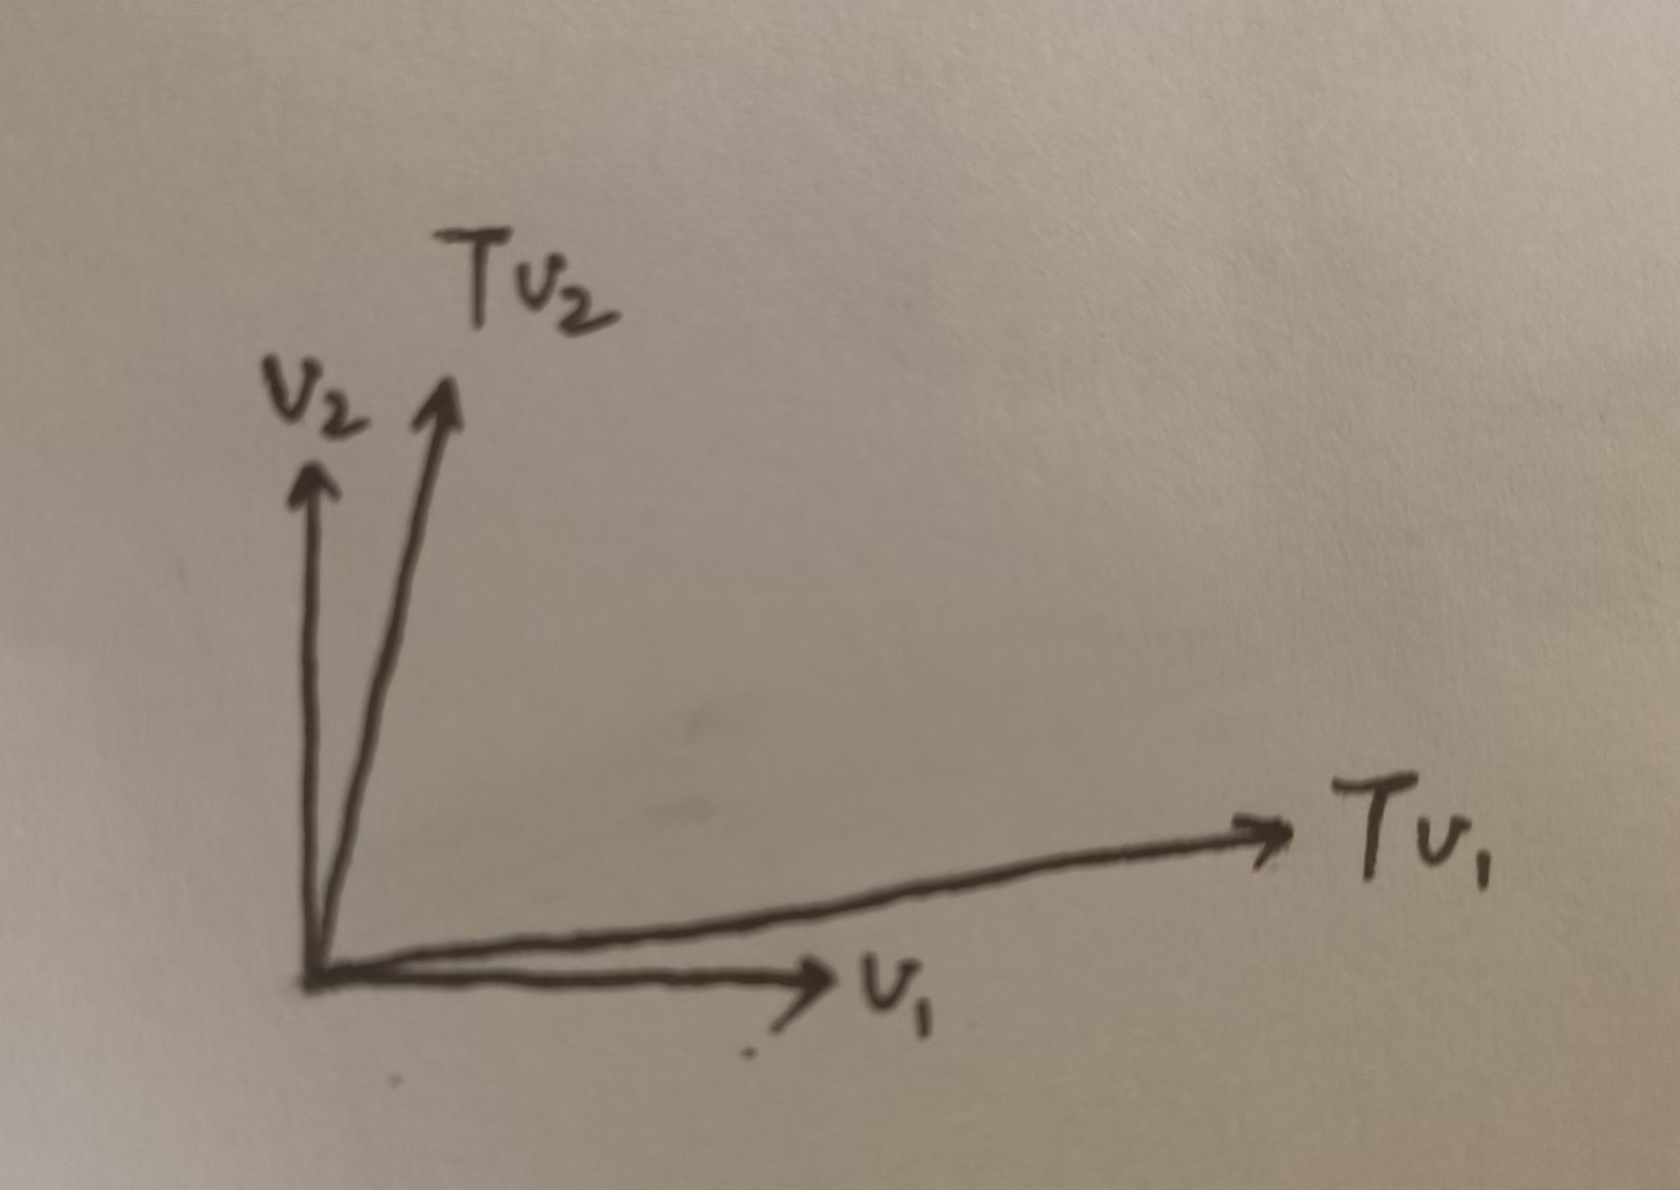
\includegraphics[width=0.5\textwidth]{figs_I2/1.jpg}
    \caption{The operator $T$ in $\mathbb{R}^2$}
    \label{fig:T_in_R2}
\end{figure}

We try to reproduce this operator by only rotations and scalings. Can we first scale $(v_1, v_2)$ and then rotate them? Or can we first rotate them and then scale? Sadly neither of these two works, as doing so would still result in a orthogonal pair $(Tv_1, Tv_2)$, which is not the case. How can we change the angle $\langle v_1, v_2\rangle$? As we would note that during a scaling with distinct scaling ratios (distinct eigenvalues), the angle between the vectors not on the scaling axis (the vectors not in the eigenspaces) would change. This is the answer — doing the ``off-axis'' scaling for $(v_1, v_2)$, shown in the figure \ref{fig:off_axis_scaling}.

\begin{figure}[H]
    \centering
    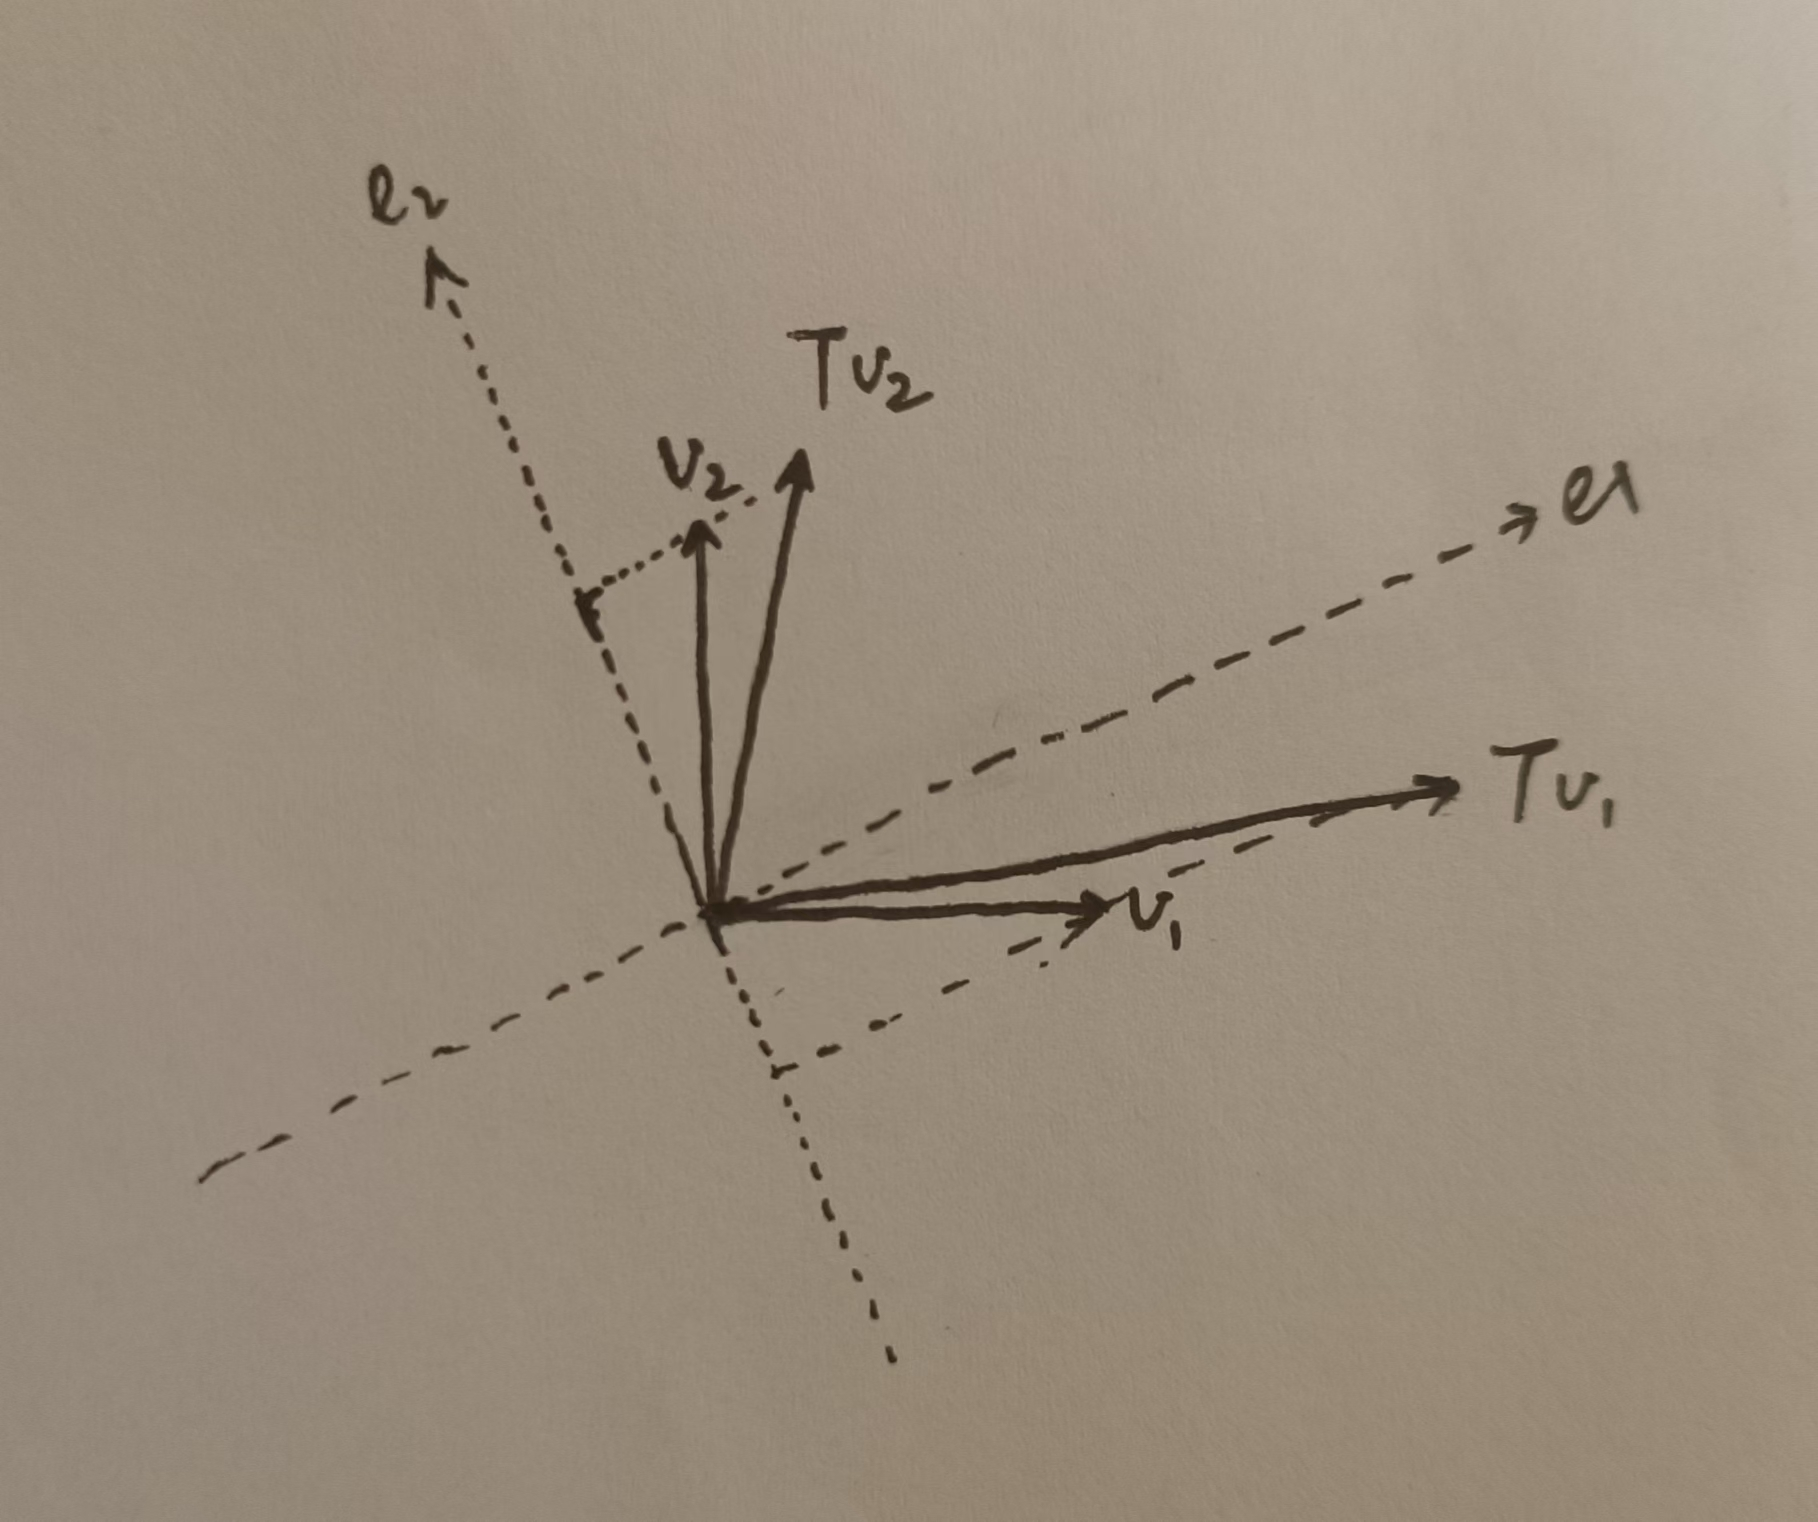
\includegraphics[width=0.5\textwidth]{figs_I2/2.jpg}
    \caption{The ``off-axis'' scaling}
    \label{fig:off_axis_scaling}
\end{figure}

Here the standard unit $(v_1, v_2)$ is distorted to $(Tv_1, Tv_2)$ as we scale $(e_1, e_2)$ to $(2e_1, e_2)$. Actually, the scaling axis $\pmb{e} = (e_1, e_2)$ here is particular, as even a tiny deviation in the orientation of $\pmb{e}$ would fail. Exactly, to drag $(v_1, v_2)$ to the target shape, we can always first only scale $e_1$ to obtain the right angle of $\langle Tv_1, Tv_2\rangle$. Then assume scaling $(e_1, e_2)\mapsto (\lambda e_1, e_2)$, with $\langle e_2, v_2 \rangle = \theta$, and thus 
$$ \frac{\Vert Tv_2 \Vert ^2}{\Vert Tv_1 \Vert ^2} = \frac{(2\sin\theta)^2 + \cos^2\theta}{(2\cos\theta)^2 + \sin^2\theta} = \frac{4\tan^2\theta+1}{4+\tan^2\theta} = r \;\;\text{ is fixed}, $$
so that the orientation of $\pmb{e}$ is determined.

Only the off-axis scaling is not enough since $T$ is not just an diagonalizable operator. What the case shown above may lacks is that the image unit $(Tv_1, Tv_2)$ is not at that position. Since the ``shape'' of the image unit is already achieved by the off-axis scaling, we can complete with only a rotation, to its right position. This is the special case of the SVD, the case for a general operator, called the \textbf{polar decomposition}. As analyzed, the polar decomposition is:
$$ T = SD $$
where $S$ is an isometry and $D$ is a diagonalizable operator (w.r.t. an orthonormal basis). 

Worthy to mention, we have furthermore the requirement for the interpretation of this decomposition, i.e., we desire that all the scaling ratios (eigenvalues) are real numbers. If not, say, $\mathcal{M}(D) = \text{diag}(z_1, \cdots, z_n)$ with complex $z_i$'s, then we can throw the imaginary compositions $\text{diag}(z_1/|z_1|, \cdots, z_n/|z_n|)$ to $S$. Better still, this way the scaling ratios are all non-negative real numbers. We then turn to study this types of operators $D$, the \text{positive operators}.

\begin{Df}{Df 8\_I2.6.8 (positive operators)}
    Suppose $V$ is a finite-dimensional inner product space over $\mathbb{F}$ and $D\in\mathcal{L}(V)$. Then $D$ is said to be \textbf{positive} if $D$ is diagonalizable w.r.t. an orthonormal basis and all its eigenvalues are non-negative real numbers. The matrices corresponding to the positive operators are called \textbf{positive-semidefinite matrices}.
\end{Df}

Obviously \textcolor{Th}{positive operators are self-adjoint.} And:
\begin{Th}{Th 8\_I2.6.8.1 (equivalent conditions for positive operators)}
    Suppose $V$ is a finite-dimensional inner product space and $D\in\mathcal{L}(V)$. Then the following are equivalent:
    \begin{compactenum}
        \item $D$ is positive;
        \item $D$ is self-adjoint and $\langle Dv, v\rangle$ is a non-negative real number for all $v\in V$;
        \item $D$ is self-adjoint and all its eigenvalues are non-negative real numbers;
        \item $D$ has a positive square root, i.e., there is a positive operator $R$ s.t. $D = R^2$;
        \item $D$ has a unique positive square root.
        \item $D$ has a self-adjoint square root;
        \item $D = R^\ast R$ for some operator $R$.
    \end{compactenum}
    \tcblower
    \textit{Pf}: Prove with cyclic implications in the order here. Now we only prove (4) $\Rightarrow$ (5). Suppose $D = R^2$, and we can prove that the behaviour of $R$ on the eigenspaces of $D$ is determined. Let $\mathcal{M}(R) = \text{diag}(\sqrt{\lambda_1},\cdots,\sqrt{\lambda_n})$ w.r.t. the orthonormal basis $(e_1, \cdots, e_n)$. Then $\mathcal{M}(D)_{\pmb{e}} = \text{diag}(\lambda_1, \cdots, \lambda_n)$. Let $v = a_1e_1+\cdots+a_ne_n$ be an eigenvector of $D$ with $Dv = \lambda v$. Then:
    $$ \sum_{i} a_i\lambda_ie_i = \sum_{i}a_iDe_i = \sum_{i}a_iR^2e_i = R^2v = Dv = \lambda v = \sum_{i}a_i\lambda e_i. $$
    And thus $a_i = 0$ whenever $\lambda \neq \lambda_i$, and $Rv$ can be written as:
    $$ Rv = \sum_{i} a_iRe_i = \sum_{i: \lambda_i = \lambda} a_iRe_i = \sum_{i: \lambda_i = \lambda} a_i\sqrt{\lambda_i}e_i = \sum_{i:\lambda_i = \lambda} a_i\sqrt{\lambda}e_i = \sqrt{\lambda}v. $$ 
\end{Th}

If an operator $T$ has the polar decomposition $T = SD$, then what $D$ should be? Since $T^\ast T = D^\ast S^\ast S D = D^\ast D = D^2$, the polar decomposition now becomes $T = S\sqrt{T^\ast T}$:

\begin{Th}{Th 8\_I2.6.9 (polar decomposition)}
    Suppose $V$ is a finite-dimensional inner product space and $T\in\mathcal{M}(V)$. Then there is an isometry $S$ such that
    $T = S\sqrt{T^\ast T}$
    \tcblower
    \textit{Pf}: The idea is to check whether the map $S_1$ s.t. $S_1\sqrt{T^\ast T}v = Tv$ for all $v$ is well-defined, and whether we can extend such $S_1$ to an isometry.
\end{Th}

If we perform polar decomposition to $T^\ast$, by $T^\ast = S\sqrt{TT^\ast}$, then we have $T = \sqrt{TT^\ast} S^\ast$. This indicates that we can also first do rotation, and then scaling, to achieve the same result of the polar decomposition. And this way we have a better understanding for the adjoint of an operator.

\subsection{SVD}
Extending the polar decomposition, SVD deals with a general map $T\in\mathcal{L}(V,W)$, where $V$ and $W$ are inner product spaces with dimensions $n$ and $m$ respectively. When $W = V$, the eigenvalues of $\sqrt{T^\ast T}$ are important, so we call them the \textbf{singular values} of $T$.

\begin{Df}{Df 8\_I2.6.10.-1 (singular values)}
    Suppose $V$ and $W$ are finite-dimensional inner product spaces and $T\in\mathcal{L}(V,W)$. Then the eigenvalues of $\sqrt{T^\ast T}$ are called the \textbf{singular values} of $T$.
\end{Df}

Different with the polar decomposition, the image unit of $T$ goes to another space. But we can still do the same for the ``virtual'' behaviour of $T$, and connect the two spaces with a (partial) isomorphism. In other word, we first do the off-axis scaling $D\in\mathcal{L}(V)$ within $V$ (so that the standard unit $\pmb{v}$ is changed to the wanted shape), and then simply send (or, copy) the resulted unit $D\pmb{v}$ to $W$ with $C\in\mathcal{L}(V,W)$ while keeping all the norms and angles of vectors, and finally complete with a isometry $S\in\mathcal{L}(W)$ to adjust to the image unit. Then the SVD has the form:
$$ T = SCD. $$
Here $D$ is positive with the eigenvalues $d_1\geq\cdots\geq d_r>0$ where $r = \dim\text{range } T$ (we use ``range'' for the ``range space'', as we will use ``$R$'' for some other operator later), and thus $\mathcal{M}(D)_{\pmb{e}} = \text{diag}(d_1,\cdots,d_r,0,\cdots,0)$ w.r.t. some orthonormal basis $\pmb{e}$. Since $C$ copies the range space of $D$ to $W$, we have $Ce_i = w_i$ ($i=1,\cdots,r$) for some known orthonormal list $(w_1,\cdots,w_r)$ (which is a sublist of an orthonormal basis $\pmb{w} = (w_1,\cdots,w_m)$). Again, what should $D$ be? Presumably $D = \sqrt{T^\ast T}$. Actually, if the SVD holds, then $T^\ast T = D^\ast C^\ast C D = D^\ast D = D^2$, where first equality is clear if you multiply the corresponding matrices (note that
$$\mathcal{M}(C)_{\pmb{e}, \pmb{w}} = 
\begin{pmatrix}
    I_r & * \\
    0 & *
\end{pmatrix}$$
where $I_r$ is the $r\times r$ identity matrix). Then the SVD is $ T = SC\sqrt{T^\ast T} $, and we state and prove it:

\begin{Th}{Th 8\_I2.6.10 (SVD)}
    Suppose $V$ and $W$ are finite-dimensional inner product spaces and $T\in\mathcal{L}(V,W)$. Then there are an isometry $S\in\mathcal{L}(W)$ such that
    $$ T = SC\sqrt{T^\ast T}, $$
    where $C$ maps one orthonormal basis of $\text{range } \sqrt{T^\ast T}$ to an orthonormal list of vectors in $W$.
    \tcblower
    \textit{Pf}: The idea is the same as the proof of the polar decomposition. \\
    Let $\mathcal{M}(\sqrt{T^\ast T})_{\pmb{e}} = \text{diag}(d_1,\cdots,d_r,0,\cdots,0)$, where
    \begin{compactenum}
        \item $r = \dim\text{range } \sqrt{T^\ast T} = \dim\text{range }T^\ast T = \dim\text{range }T$,
        \item $d_1\geq\cdots\geq d_r > 0$, and
        \item $\pmb{e} = (e_1,\cdots,e_r,\cdots,e_n)$ an orthonormal basis of $V$.
    \end{compactenum}
    Then $(e_1,\cdots,e_r)$ is an orthonormal basis of $\text{range } \sqrt{T^\ast T}$. Let $\pmb{w} = (w_1,\cdots,w_r,\cdots,w_m)$ be an orthonormal basis of $W$, then define $C$ as:
    $$ \begin{cases}
        Ce_i = w_i \quad (i\leq r) \\
        Ce_i = 0 \quad (i>r)
    \end{cases} $$
    Then the operator $S$ defined as $S \left(C\sqrt{T^\ast T}v\right) = Tv$ is an isometry. To check this, we first show that $C\sqrt{T^\ast T}v_1 = C\sqrt{T^\ast T}v_2$ implies $Tv_1 = Tv_2$ so that $S$ is well-defined on the range of $C\sqrt{T^\ast T}$; then we show that on $\text{range } C\sqrt{T^\ast T}$, $S$ preserves the norms of vectors so that it can be extended to an isometry.\\
    Assume $C\sqrt{T^\ast T}v_1 = C\sqrt{T^\ast T}v_2$. Since $C$ is the ``identity'' on the range of $\sqrt{T^\ast T}$, we have $\sqrt{T^\ast T}v_1 = \sqrt{T^\ast T}v_2$, and thus, as have been proved in the polar decomposition, $Tv_1 = Tv_2$. Next, 
    $$ \Vert S(C\sqrt{T^\ast T}v)\Vert = \Vert Tv\Vert = \Vert \sqrt{T^\ast T}v\Vert = \Vert C\sqrt{T^\ast T}v\Vert. $$
    Hence $S$ is an isometry and we complete the proof.
\end{Th}

When $W = V$, $C$ maps $(e_1,\cdots,e_r)$ to some orthonormal list in $V$. Since the behaviour of $C$ on $(\text{range}\sqrt{T^\ast T})^\perp$ does not matter, we may say that $C$ is an isometry, and then the SVD just reduces to the polar decomposition.

\subsection{The Matrix Representation of SVD}
Suppose $T\in\mathcal{L}(V, W)$, $\dim V = n$, $\dim W = m$. Then $T = SCD$ and $D = \sqrt{T^\ast T}$. Given the standard bases $\pmb{v}$ of $V$ and $\pmb{w}$ of $W$, we then derive the matrix representation of SVD, which is seen in most of the textbook of matrix theory.

Let 
$$ \mathcal{M}(D)_{\pmb{e},\pmb{e}} = 
\begin{bmatrix}
    D_r & O \\
    O & O
\end{bmatrix}_{n\times n} \qquad \mathcal{M}(C)_{\pmb{e},\pmb{w}} = 
\begin{bmatrix}
    I_r & O \\
    O & O
\end{bmatrix}_{m\times n} $$
where $D_r = \text{diag}(d_1,\cdots,d_r)$ ($d_1\geq\cdots\geq d_r>0$), $I_r$ is the $r\times r$ identity matrix, and $O$ represent some zero matrices. Then 
$$ \mathcal{M}(CD)_{\pmb{e,w}} = 
\begin{bmatrix}
    D_r & O_{r\times (n-r)} \\
    O_{(m-r)\times r} & O_{(m-r)\times (n-r)} 
\end{bmatrix}
$$ 
This is beautiful and we want it appears in our result. Since $\pmb{e}$ is beforehand unknown, we suppose $R$ is the isometry that maps $\pmb{v}$ to $\pmb{e}$: $R\pmb{v} = \pmb{e}$. Then:
$$ \begin{aligned}
    \mathcal{M}(T)_{\pmb{v,w}} &= \mathcal{M}(SCD)_{\pmb{v,w}} = \mathcal{M}(S)_{\pmb{w,w}}\mathcal{M}(C)_{\pmb{v,w}}\mathcal{M}(D)_{\pmb{v,v}} \\
    &=\mathcal{M}(S)_{\pmb{w,w}}\Big[\mathcal{M}(C)_{\pmb{e,w}}\mathcal{M}(R)^\ast_{\pmb{v,v}}\Big] \Big[\mathcal{M}(R)_{\pmb{v,v}}\mathcal{M}(D)_{\pmb{e,e}}\mathcal{M}(R)_{\pmb{v,v}}^\ast\Big] \\
    &= \mathcal{M}(S)_{\pmb{w,w}}\mathcal{M}(C)_{\pmb{e,w}}\mathcal{M}(D)_{\pmb{e,e}}\mathcal{M}(R)^{\ast}_{\pmb{v,v}} = \mathcal{M}(S)_{\pmb{w,w}}\mathcal{M}(CD)_{\pmb{e,w}}\mathcal{M}(R)^{\ast}_{\pmb{v,v}}
\end{aligned}
$$
This is just:
$$ A = F\Sigma E^\ast, $$
where $E$ and $F$ are unitary matrices of order $n$ and $m$ respectively, and 
$$ \Sigma = 
\begin{bmatrix}
    D_r & O_{r\times (n-r)} \\
    O_{(m-r)\times r} & O_{(m-r)\times (n-r)} 
\end{bmatrix} $$
Then it comes to computing $E$ and $F$. Of course $E = \mathcal{M}(R)_{\pmb{v,v}} = [e_1\cdots e_n]$, and the first $r$ columns of $F$ are $(Sw_1,\cdots,Sw_r)$. Since $Sw_1 = SCe_1 = SCD(e_1/d_1) = T(e_1/d_1) = Te_1/d_1$, we conplete the computation, with the steps concluded in the theorem below:

\begin{Th}{Th 8\_I2.6.10.1 (compute the SVD)}
    \begin{compactenum}
        \item Suppose $A\in\mathbb{F}^{m,n}$. Then the eigenvalues of $A^\ast A$ are $\lambda_1,\cdots,\lambda_r,\underbrace{0,\cdots,0}_{n-r}$ where all these $\lambda_i$'s are positive real numbers and $r = \text{rank}(A)$. 
        \item The eigenspaces of $A^\ast A$ sums to the whole space, and different eigenspaces are mutually orthogonal, thus we can solve the orthonormal eigenbasis $(e_1,\cdots,e_r,e_{r+1},\cdots,e_n)$ corresponding to $\lambda_1,\cdots,\lambda_r,\underbrace{0,\cdots,0}_{n-r}$.
        \item Let $f_i = Ae_i/\sqrt{\lambda_i}$ ($i=1,\cdots,r$). Then $(f_1,\cdots,f_r)$ is an orthonormal list of vectors, and thus we can extend it to an orthonormal basis $(f_1, \cdots, f_r, f_{r+1}, \cdots, f_m)$.
        \item As a result,
        $$ A = F\,\Sigma\, E^\ast, $$
        where $F = (f_1,\cdots,f_m)$, $E = (e_1,\cdots, e_n)$ are unitary, and
        $$ \Sigma = \begin{bmatrix}
            D_r & O \\
            O & O
        \end{bmatrix}_{m\times n}\qquad D_r = \begin{bmatrix}
            \sqrt{\lambda_1} & & \\
            & \ddots & \\
            & & \sqrt{\lambda_r}
        \end{bmatrix}, $$
        with the ``$O$'' represent some zero matrices of proper sizes. \textcolor{Df}{These $\sqrt{\lambda_i}$'s are called the singular values of $A$.}
    \end{compactenum}
\end{Th}
\end{document}